\chapter{Metode Penelitian}

Bab ini menjelaskan tahapan yang ditempuh untuk menjawab tujuan penelitian, mulai dari 
penyiapan data hingga implementasi sistem pemantauan. Uraian disusun mengikuti urutan kerja 
penelitian, yaitu pengumpulan dan penyiapan data, pelatihan dan evaluasi model, penyetelan 
model terpilih, lalu perancangan sistem. Tiap tahap dijelaskan pada subbab tersendiri agar 
prosedurnya dapat diikuti dan direproduksi.

\section{Gambaran Umum Penelitian}
\label{sec:gambaran_umum}

Penelitian ini dilaksanakan melalui tujuh tahap berurutan yang membentuk satu
alur dari penyediaan data hingga sistem yang berjalan, seperti ditunjukkan pada Gambar
\ref{fig:alur_penelitian}. Tahap pertama adalah pengumpulan data citra dari \textit{stream} kamera CCTV
kawasan Malioboro. Citra yang terkumpul kemudian dianotasi pada tahap kedua
menggunakan pendekatan semiotomatis untuk menghasilkan label sembilan kelas objek.
Tahap ketiga membersihkan anotasi dari kesalahan geometris dan membagi data menjadi
himpunan latih, validasi, dan uji. Tahap keempat melatih delapan varian model YOLOv8
dan YOLO11 dengan konfigurasi identik untuk membandingkannya secara terkontrol. Tahap
kelima mengevaluasi performa tiap varian menggunakan sejumlah metrik dan memilih
model dengan keseimbangan akurasi serta kecepatan terbaik. Tahap keenam menyetel
resolusi citra masukan model terpilih untuk mengoptimasi performanya. Tahap ketujuh
menerapkan model hasil penyetelan ke dalam sistem pemantauan berbasis web yang
memproses video secara \textit{real-time} dan menyajikan informasi kepadatan beserta
notifikasinya.

\begin{figure}[h]
    \centering
    \begin{tikzpicture}[
        node distance=1.0cm,
        tahap/.style={rectangle, rounded corners, draw, text width=8.5cm, align=center, minimum height=0.9cm, fill=gray!8, font=\small},
        panah/.style={-{Latex[length=2mm]}, thick}
    ]
        \node (t1) [tahap] {Pengumpulan data citra dari \textit{stream} CCTV kawasan Malioboro};
        \node (t2) [tahap, below=of t1] {Anotasi semiotomatis untuk sembilan kelas objek};
        \node (t3) [tahap, below=of t2] {Pembersihan anotasi dan pembagian \textit{train}, \textit{validation}, \textit{test}};
        \node (t4) [tahap, below=of t3] {Pelatihan dan perbandingan delapan varian YOLOv8 dan YOLO11};
        \node (t5) [tahap, below=of t4] {Evaluasi metrik dan pemilihan model terbaik};
        \node (t6) [tahap, below=of t5] {Penyetelan resolusi citra masukan model terpilih};
        \node (t7) [tahap, below=of t6] {Implementasi model pada sistem pemantauan berbasis web};
        \draw[panah] (t1) -- (t2);
        \draw[panah] (t2) -- (t3);
        \draw[panah] (t3) -- (t4);
        \draw[panah] (t4) -- (t5);
        \draw[panah] (t5) -- (t6);
        \draw[panah] (t6) -- (t7);
    \end{tikzpicture}
    \caption{Alur tahapan penelitian.}
    \label{fig:alur_penelitian}
\end{figure}

Ketujuh tahap tersebut bersifat berurutan, yaitu keluaran satu tahap menjadi
masukan bagi tahap berikutnya. Kualitas anotasi pada tahap kedua dan ketiga menetapkan
batas atas performa yang dapat dicapai model pada tahap keempat, sedangkan performa
model menentukan keandalan informasi kepadatan yang disajikan sistem pada tahap
ketujuh. Karena keterkaitan tersebut, tahap penyiapan data dan pelatihan model diuraikan
secara rinci pada subbab-subbab berikutnya sebelum perancangan sistem dibahas pada
bagian akhir bab ini.

\section{Alat dan Bahan Tugas Akhir}
\label{sec:alat_bahan}

Subbab ini menjelaskan perangkat keras dan perangkat lunak yang digunakan sepanjang 
penelitian. Spesifikasi dicantumkan agar tahap pelatihan dan pengujian dapat diulang 
pada lingkungan yang setara. Pemisahan antara lingkungan pelatihan berperforma tinggi dan 
perangkat penerapan yang terbatas juga ditegaskan di sini, karena keduanya berperan berbeda 
dalam menilai akurasi dan kecepatan model.

\subsection{Perangkat Keras}

Pelatihan model dilakukan pada lingkungan komputasi performa tinggi 
(\textit{high-performance computing}, HPC) milik Departemen Teknik Elektro dan Teknologi 
Informasi, Fakultas Teknik, Universitas Gadjah Mada. Lingkungan ini menyediakan GPU NVIDIA 
Tesla V100-SXM2 dengan memori 32 GB, yang memungkinkan pelatihan seluruh varian model 
termasuk ukuran \textit{large} tanpa kendala keterbatasan memori. Kapasitas memori sebesar 
itu penting karena pelatihan memakai \textit{batch size} otomatis yang menyesuaikan beban 
GPU, sehingga varian besar tetap dapat dilatih tanpa kehabisan memori.

Perancangan dan pengujian sistem dilakukan pada laptop dengan prosesor AMD Ryzen 5 5600H, 
GPU NVIDIA GeForce GTX 1650 bermemori 4 GB, RAM 16 GB (2 $\times$ 8 GB DDR4-3200), dan 
sistem operasi Windows 11 Home Single Language 64-bit. Spesifikasi ini mewakili kelas 
perangkat dengan sumber daya terbatas sebagai target penerapan \textit{real-time}. Pemilihan 
perangkat kelas ini disengaja agar pengukuran kecepatan inferensi mencerminkan kondisi 
penerapan yang realistis, bukan performa pada server kelas atas.

\subsection{Perangkat Lunak}

Pelatihan dan inferensi model menggunakan pustaka Ultralytics yang menyediakan 
implementasi YOLOv8 dan YOLO11 di atas \textit{framework} PyTorch. Proses anotasi data 
dilakukan pada platform Roboflow, sedangkan pembacaan dan pemrosesan \textit{frame} 
video dilakukan dengan pustaka OpenCV. Versi perangkat lunak utama yang digunakan pada 
lingkungan pelatihan dirangkum pada Tabel \ref{tab:perangkat_lunak}.

\begin{table}[h]
    \centering
    \caption{Versi perangkat lunak utama yang digunakan pada lingkungan pelatihan.}
    \label{tab:perangkat_lunak}
    \begin{tabular}{|l|l|}
        \hline
        \textbf{Perangkat lunak} & \textbf{Versi} \\
        \hline \hline
        Python & 3.10.12 \\
        PyTorch & 2.2.0a0+81ea7a4 \\
        CUDA & 12.3 \\
        Ultralytics & 8.4.63 \\
        OpenCV (cv2) & 4.9.0 \\
        Roboflow & Platform anotasi berbasis web \\
        \textit{Backend} sistem web & FastAPI (Python) \\
        \hline
        \textit{Frontend} sistem web & React, Vite, Tailwind \\
        \hline
        Basis data riwayat deteksi & SQLite \\
        \hline
    \end{tabular}
\end{table}

\section{Pengumpulan Data}
\label{sec:pengumpulan_data}

Pengumpulan data bertujuan membangun kumpulan citra primer yang mewakili kondisi nyata 
kawasan Malioboro sebagai bahan pelatihan dan pengujian model deteksi. Subbab ini 
menjelaskan sumber dan mekanisme pengambilan citra, penjadwalan pengambilan untuk 
memperoleh variasi kondisi, serta penyaringan citra yang tidak layak digunakan.

\subsection{Sumber dan Mekanisme Pengambilan \textit{Frame}}

Data primer penelitian berupa citra yang diambil dari \textit{stream} video langsung 22 
kamera CCTV publik di kawasan Malioboro yang dikelola Pemerintah Kota Yogyakarta. 
\textit{Stream} video disediakan dalam format \textit{HTTP Live Streaming} (HLS) melalui 
berkas \textit{playlist} berekstensi \texttt{.m3u8}, sehingga setiap kamera dapat diakses 
sebagai sumber video daring. Akses daring ini memungkinkan pengambilan citra tanpa pemasangan 
perangkat tambahan di lapangan, sekaligus memastikan data berasal dari kondisi nyata 
kawasan.

Pengambilan citra dilakukan secara otomatis menggunakan program yang ditulis dengan 
bahasa Python. Program memiliki penjadwal internal sendiri, yaitu dijalankan satu kali 
lalu menunggu hingga slot waktu berikutnya tanpa bergantung pada penjadwal sistem 
eksternal. Pada setiap slot, program mengambil satu \textit{frame} dari tiap kamera.

Pengambilan satu \textit{frame} dari \textit{stream} HLS memerlukan penanganan khusus karena 
\textit{stream} menyimpan \textit{buffer} yang berisi \textit{frame} lama. Program membuka 
\textit{stream}, menunggu dua detik agar koneksi stabil, membuang 30 \textit{frame} pertama 
dari \textit{buffer}, lalu mengambil satu \textit{frame} terkini. Jika pengambilan 
gagal, proses diulang hingga tiga kali sebelum kamera tersebut ditandai gagal. Setiap 
\textit{frame} yang berhasil disimpan dalam format JPEG dengan kualitas 92, dan diberi 
nama berkas yang memuat nomor kamera, tanggal, dan waktu pengambilan, sehingga tiap 
citra dapat diidentifikasi sumber serta waktunya tanpa berkas catatan terpisah. Prosedur 
lengkap pengambilan satu \textit{frame} dari \textit{stream} HLS dirangkum pada Algoritma 
\ref{alg:capture}.

\begin{algorithm}[h]
    \caption{Pengambilan satu \textit{frame} terkini dari \textit{stream} HLS.}
    \label{alg:capture}
    \begin{algorithmic}[1]
        \Require URL \textit{playlist} \texttt{.m3u8} dari satu kamera
        \Ensure satu \textit{frame} terkini, atau status gagal
        \For{$i \gets 1$ \textbf{sampai} $3$}
            \State buka \textit{stream} dari URL
            \State tunggu 2 detik agar koneksi stabil
            \State buang 30 \textit{frame} pertama dari \textit{buffer}
            \State $f \gets$ ambil satu \textit{frame} terkini
            \If{$f$ berhasil diambil}
                \State simpan $f$ sebagai berkas JPEG kualitas 92
                \State \textbf{kembalikan} $f$
            \EndIf
            \State tutup \textit{stream}
        \EndFor
        \State tandai kamera sebagai gagal
    \end{algorithmic}
\end{algorithm}

\subsection{Penjadwalan dan Variasi Kondisi}

Pengumpulan data berlangsung selama satu pekan, yaitu 30 April hingga 6 Mei 2026. Rentang 
waktu ini dipilih agar data mencakup variasi kondisi antarhari, antarjam, dan antarcuaca, 
sehingga model dilatih pada keragaman situasi yang mendekati kondisi nyata. Variasi tersebut 
penting karena kepadatan dan pencahayaan di Malioboro berubah tajam antara dini hari yang 
sepi dan malam hari yang ramai, sehingga model perlu melihat rentang kondisi yang luas.

Dalam satu hari, pengambilan dilakukan pada 11 slot waktu yang mewakili rentang kepadatan 
dan pencahayaan, mulai dari dini hari yang sepi, meningkat sepanjang siang, hingga memuncak 
pada sore dan malam hari sesuai karakter kawasan wisata Malioboro. Pembagian slot setiap dua 
jam menyeimbangkan cakupan sepanjang hari dengan jumlah citra yang masih wajar untuk 
dianotasi. Rincian slot ditunjukkan pada Tabel \ref{tab:slot_pengumpulan}.

\begin{table}[h]
    \centering
    \caption{Slot waktu pengambilan citra dalam satu hari.}
    \label{tab:slot_pengumpulan}
    \begin{tabular}{|c|l|l|}
        \hline
        \textbf{Pukul} & \textbf{Label Slot} & \textbf{Keterangan Kondisi} \\
        \hline \hline
        00.00 & \textit{midnight} & keramaian larut malam mulai menurun \\
        02.00 & \textit{dawn} & kondisi paling sepi \\
        06.00 & \textit{early\_morning} & aktivitas masih rendah \\
        08.00 & \textit{morning} & aktivitas pagi meningkat \\
        10.00 & \textit{midmorning} & kunjungan wisatawan meningkat \\
        12.00 & \textit{noon} & keramaian siang \\
        14.00 & \textit{afternoon} & keramaian siang berlanjut \\
        16.00 & \textit{late\_afternoon} & keramaian menjelang sore \\
        18.00 & \textit{evening} & awal puncak keramaian malam \\
        20.00 & \textit{night} & puncak keramaian malam \\
        22.00 & \textit{late\_night} & keramaian mulai menurun \\
        \hline
    \end{tabular}
\end{table}

Dengan 11 slot, 22 kamera, dan 7 hari, jumlah \textit{frame} yang ditargetkan secara 
teoretis adalah 1.694. Sebagian percobaan pengambilan gagal akibat gangguan koneksi 
\textit{stream}, sehingga jumlah citra yang berhasil dikumpulkan adalah 1.581. Seluruh citra 
tersebut digunakan tanpa penyaringan lebih lanjut, lalu dilanjutkan ke tahap anotasi.

\section{Anotasi Data}
\label{sec:anotasi_data}

Anotasi bertujuan memberi label berupa kotak pembatas dan kelas pada setiap objek di 
dalam citra. Subbab ini menjelaskan strategi anotasi yang dipilih akibat keterbatasan 
waktu, perbandingan beberapa pendekatan pelabelan otomatis untuk menentukan 
\textit{baseline}, serta anotasi manual dan koreksi yang melengkapinya. Seluruh proses 
anotasi dikerjakan pada platform Roboflow.

\subsection{Strategi Anotasi Semiotomatis}

Rencana awal penelitian adalah menganotasi seluruh citra secara manual agar kualitas 
label terjaga. Setelah 329 citra selesai dianotasi manual, waktu yang tersedia dinilai 
tidak mencukupi untuk menyelesaikan seluruh 1.581 citra dengan cara yang sama dalam 
jadwal penyusunan skripsi. Oleh karena itu, sisa 1.252 citra dianotasi menggunakan 
pendekatan semiotomatis, yaitu pelabelan otomatis oleh model \textit{pretrained} yang 
kemudian diperiksa dan dikoreksi secara manual \cite{tenckhoff2025feedback}.

Dengan pembagian tersebut, 329 citra hasil anotasi manual digunakan sebagai data dengan 
label yang dianggap bersih, sedangkan 1.252 citra hasil anotasi semiotomatis digunakan 
sebagai data latih. Pemisahan ini menempatkan label yang paling tepercaya pada himpunan yang 
dipakai untuk mengukur performa, sementara himpunan latih boleh memuat sedikit 
ketidaksempurnaan label tanpa membiaskan evaluasi. Pembagian ke dalam himpunan latih, 
validasi, dan uji diuraikan pada Subbab \ref{sec:pembersihan_pembagian}.

\subsection{Perbandingan Pendekatan Pelabelan Otomatis}

Tahap pelabelan otomatis memerlukan model dasar yang menghasilkan kotak pembatas awal. 
Tiga kombinasi model diuji pada 1.252 citra latih untuk menentukan pilihan terbaik. 
Pada ketiga kombinasi, kelas bajaj dideteksi oleh model YOLOv12s yang telah dilatih pada 
dataset BMD-45 \cite{sharma2025bmd}, sedangkan kelas lain dideteksi oleh model dasar yang 
berbeda, yaitu SAM3 \cite{carion2025sam3}, YOLO11x, atau YOLOv8x. Pelabelan dengan SAM3 
dilakukan melalui layanan Roboflow API. Jumlah \textit{instance} hasil tiap kombinasi 
dirangkum pada Tabel \ref{tab:perbandingan_autolabel}.

\begin{table}[h]
    \centering
    \caption{Jumlah \textit{instance} hasil tiga kombinasi pelabelan otomatis pada 1.252 citra latih.}
    \label{tab:perbandingan_autolabel}
    \begin{tabular}{|l|r|r|r|}
        \hline
        % \textbf{Kelas} & \textbf{SAM3} & \textbf{YOLO11x} & \textbf{YOLOv8x} \\
        \textbf{Kelas} & \multicolumn{1}{|c|}{\textbf{SAM3}} & \multicolumn{1}{c|}{\textbf{YOLO11x}} & \multicolumn{1}{c|}{\textbf{YOLOv8x}} \\
        \hline \hline
        andong & 0 & 0 & 0 \\
        bajaj & 112 & 112 & 112 \\
        becak & 0 & 0 & 0 \\
        sepeda & 3.916 & 277 & 265 \\
        bus & 549 & 114 & 123 \\
        mobil & 11.964 & 1.789 & 1.821 \\
        motor & 32.074 & 1.894 & 2.124 \\
        orang & 81.000 & 7.784 & 9.803 \\
        truk & 619 & 276 & 250 \\
        \hline
        \textbf{Total} & \textbf{130.234} & \textbf{12.246} & \textbf{14.498} \\
        \hline
    \end{tabular}
\end{table}

Dua kelas, yaitu andong dan becak, tidak terdeteksi sama sekali oleh ketiga kombinasi 
karena tidak tersedia pada model dasar mana pun, sementara bajaj menghasilkan jumlah 
yang sama, yaitu 112, karena memakai model yang identik. Perbedaan utama terletak pada 
kelas umum. Kombinasi berbasis SAM3 menghasilkan 130.234 \textit{instance}, hampir 
sembilan kali lipat dibanding YOLOv8x, dengan kelas orang saja mencapai 81.000. SAM3 
dirancang untuk menemukan seluruh \textit{instance} dari suatu konsep sekaligus, sehingga 
pada citra yang padat cenderung menghasilkan deteksi yang sangat banyak dan didominasi 
\textit{false positive}. Akibatnya, biaya koreksi manualnya justru lebih besar daripada 
manfaatnya.

Sebagian dari selisih jumlah \textit{instance} ini berasal dari konfigurasi yang berbeda. 
Pelabelan SAM3 melalui Roboflow API menggunakan ambang keyakinan (\textit{confidence 
threshold}) bawaan sebesar 0,25, lebih rendah dibanding ambang 0,35 yang digunakan pada 
YOLO11x dan YOLOv8x, sehingga SAM3 mempertahankan lebih banyak deteksi berkeyakinan rendah 
yang pada model lain sudah disaring. Namun, perbedaan ambang ini hanya menjelaskan 
sebagian dari selisih sembilan kali lipat yang teramati, dan tidak menjelaskan mengapa 
selisih tersebut jauh lebih besar pada kelas umum yang padat di kawasan Malioboro 
dibanding kelas yang lebih jarang muncul, seperti bus dan truk pada Tabel 
\ref{tab:perbandingan_autolabel}.

Penjelasan yang lebih mendasar terletak pada perbedaan arsitektural antara model deteksi 
seperti YOLO dan model segmentasi \textit{promptable} seperti SAM3. Dalam mode otomatis 
tanpa prompt spesifik per objek, SAM menempatkan kisi titik (\textit{grid of points}) 
yang padat di seluruh citra sebagai prompt implisit dan menghasilkan satu \textit{mask} 
untuk tiap titik, sebuah strategi yang tidak memiliki mekanisme pemandu lokalisasi 
sebagaimana \textit{region proposal} atau \textit{anchor} pada detektor konvensional, 
sehingga rawan menghasilkan \textit{mask} berlebih dan redundan pada citra yang padat 
objek \cite{gao2026pmgsam}. Pada objek kecil yang berkelompok rapat, seperti orang 
dan motor di kawasan Malioboro, kepadatan kisi titik yang seragam ini cenderung 
menghasilkan banyak \textit{mask} tumpang tindih untuk objek yang sama atau objek yang 
berdekatan, alih-alih satu \textit{mask} per objek yang bersih. Keterbatasan ini diperparah 
oleh \textit{encoder} berbasis \textit{Vision Transformer} pada SAM \cite{kirillov2023segment}, 
yang memampatkan citra ke ruang representasi beresolusi rendah sehingga detail batas objek 
kecil berisiko hilang sebelum mencapai tahap dekode \textit{mask}, sebuah keterbatasan yang 
juga ditegaskan oleh kajian terhadap SAM pada tugas segmentasi objek kecil dan struktur 
detail \cite{yu2025granular}. Detektor seperti 
YOLO, sebaliknya, dilatih khusus untuk regresi kotak pembatas per kelas objek dengan 
penekan non-maksimum (\textit{non-maximum suppression}) berbasis kelas yang membatasi 
jumlah kotak akhir per objek, sehingga lebih sesuai untuk ekstraksi kotak pembatas pada 
objek kecil yang padat dibanding strategi \textit{segment-everything} milik SAM.

Kombinasi YOLOv8x dipilih sebagai \textit{baseline}. Dibandingkan YOLO11x, YOLOv8x 
bersifat lebih agresif, terlihat dari jumlah \textit{instance} yang lebih banyak, yaitu 
14.498 berbanding 12.246. Sifat agresif ini menguntungkan pada tahap awal pelabelan karena 
menghapus \textit{false positive} lebih cepat daripada menambahkan deteksi yang terlewat 
secara manual. SAM3 tidak dipilih karena tingkat deteksi berlebihnya terlalu tinggi, baik 
akibat ambang keyakinan yang lebih rendah maupun akibat karakteristik arsitekturalnya, 
sehingga \textit{noise} yang dihasilkan tidak sebanding dengan waktu koreksi yang 
diperlukan.

Pemilihan ini berangkat dari asimetri biaya koreksi manual. Menghapus \textit{false 
positive} hanya menuntut anotator mengenali dan membuang kotak yang keliru, sedangkan 
menambahkan deteksi yang terlewat menuntut anotator menemukan objek yang luput di seluruh 
citra, pekerjaan yang jauh lebih lambat dan rawan terabaikan. Karena itu, model dasar yang 
sedikit terlalu agresif lebih disukai daripada yang terlalu konservatif, sepanjang tingkat 
\textit{false positive}-nya masih wajar. SAM3 berada di ujung yang berlawanan, karena 
tingkat deteksi berlebihnya begitu tinggi sehingga keuntungan dari kelengkapan deteksi 
tertutup oleh beban memverifikasi puluhan ribu kotak tambahan. YOLOv8x menempati titik 
tengah yang paling praktis, yaitu cukup agresif untuk meminimalkan objek terlewat tanpa 
membanjiri anotator dengan \textit{noise}.

\subsection{Anotasi Manual dan Koreksi}
 
Hasil pelabelan otomatis melengkapi sebagian besar kelas, tetapi belum mencakup andong dan 
becak yang tidak terdeteksi oleh model dasar mana pun. Kedua kelas tersebut dianotasi secara 
manual penuh pada citra latih. Penambahan manual ini diperlukan karena andong dan becak tidak 
memiliki padanan kelas pada model \textit{pretrained}, sehingga tidak mungkin muncul dari 
pelabelan otomatis.
 
Selain penambahan dua kelas tersebut, hasil \textit{baseline} YOLOv8x ditinjau dan 
dikoreksi secara manual semaksimal mungkin. Koreksi ini penting karena kualitas label pada 
data latih menjadi batas atas performa yang dapat dicapai model. Gambar 
\ref{fig:contoh_misspredict} menunjukkan salah satu contoh kesalahan, yaitu tiga bangku 
taman yang terdeteksi sebagai objek (\textit{false positive}).
 
\begin{figure}[h]
    \centering
    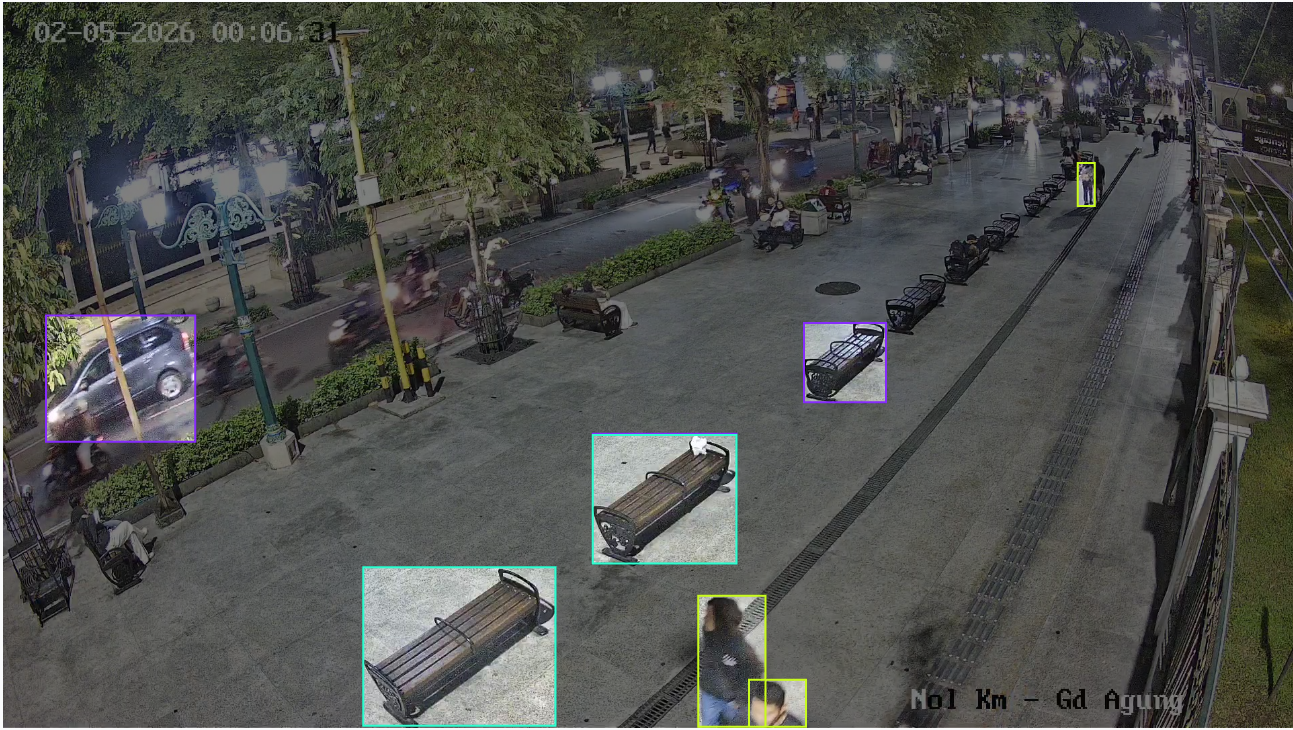
\includegraphics[width=0.8\textwidth]{contents/chapter-3/contoh_misspredict.png}
    \caption{Contoh kesalahan deteksi tiga bangku taman yang terdeteksi sebagai objek.}
    \label{fig:contoh_misspredict}
\end{figure}
 
Selain contoh pada gambar tersebut, penulis menemukan beberapa pola kesalahan yang 
berulang. Kotak pembatas kelas bus dan truk sering tumpang tindih pada objek yang sama. 
Kelas bajaj kadang terlabeli sebagai truk, sedangkan becak terkadang terdeteksi sebagai 
motor. Latar belakang citra juga beberapa kali terdeteksi sebagai salah satu dari sembilan 
kelas. Seluruh kesalahan tersebut diperbaiki secara manual, baik dengan menghapus deteksi 
yang keliru, memperbaiki label kelas, maupun menyesuaikan kotak pembatas.
 
Anotasi manual dan koreksi ini mengubah jumlah dan komposisi label dari hasil 
\textit{baseline}. Perubahan tersebut mencakup penambahan \textit{instance} kelas andong dan 
becak sekaligus pengurangan deteksi keliru pada kelas lain. Distribusi akhir setelah 
pembersihan beserta pembagian data diuraikan pada subbab \ref{sec:pembersihan_pembagian}.

\section{Pembersihan dan Pembagian Dataset}
\label{sec:pembersihan_pembagian}

Sebelum digunakan untuk pelatihan dan evaluasi, anotasi dibagi ke dalam tiga himpunan lalu 
dibersihkan dari kesalahan geometris. Urutan ini dipilih agar pembagian dilakukan lebih dulu 
berdasarkan asal anotasi, baru pembersihan diterapkan seragam pada tiap himpunan. Subbab ini 
menjelaskan pembagian data, proses pembersihan anotasi, serta distribusi kelas akhir beserta 
ketidakseimbangannya.

\subsection{Pembagian \textit{Train}, \textit{Validation}, dan \textit{Test}}

Data dibagi ke dalam tiga himpunan, yaitu latih (\textit{train}), validasi 
(\textit{validation}), dan uji (\textit{test}). Pembagian mengikuti cara anotasi yang 
dijelaskan pada subbab \ref{sec:anotasi_data}. Sebanyak 1.252 citra hasil anotasi 
semiotomatis digunakan sebagai himpunan latih, sedangkan 329 citra hasil anotasi manual 
dibagi menjadi 165 citra validasi dan 164 citra uji.

Penempatan seluruh citra ber-anotasi manual pada himpunan validasi dan uji dilakukan 
dengan sengaja. Kedua himpunan tersebut menjadi acuan pengukuran performa model, sehingga 
keduanya perlu memiliki label yang andal. Dengan label manual pada validasi dan uji, 
performa model diukur terhadap acuan yang tepercaya, terlepas dari kemungkinan kesalahan 
yang masih tersisa pada label semiotomatis di himpunan latih.

\subsection{Pembersihan Geometris Anotasi}

Anotasi dibersihkan dari kotak pembatas yang tidak valid secara geometris menggunakan 
lima filter. Kotak yang sangat kecil disaring karena objek dengan luas di bawah 0,1\% 
luas citra setara dengan kurang dari 20$\times$20 piksel setelah citra diskala ke 
640$\times$640, sehingga terlalu kecil untuk dipelajari dan sejalan dengan perhatian 
terhadap objek berukuran sangat kecil pada COCO \cite{lin2014coco}. Kotak yang menutupi 
lebih dari 90\% luas citra disaring sebagai kesalahan anotasi, sedangkan kotak dengan 
rasio sisi yang ekstrem, baik terlalu tipis maupun terlalu lebar, juga disingkirkan. 
Rincian ambang tiap filter ditunjukkan pada Tabel \ref{tab:filter_cleaning}.

\begin{table}[h]
    \centering
    \caption{Filter pembersihan kotak pembatas.}
    \label{tab:filter_cleaning}
    \begin{tabular}{|p{5.8cm}|c|p{5cm}|}
        \hline
        % \centering \textbf{Kriteria} & \textbf{Ambang} & \textbf{Tindakan} \\
        \textbf{Kriteria} & \textbf{Ambang} & \textbf{Tindakan} \\
        \hline \hline
        Luas ternormalisasi minimum & 0,001 & buang kotak $<$ 0,1\% luas citra \\
        \hline
        Luas ternormalisasi maksimum & 0,90 & buang kotak $>$ 90\% luas citra \\
        \hline
        Rasio sisi minimum & 0,15 & buang kotak terlalu tipis (lebar/tinggi $<$ 0,15) \\
        \hline
        Rasio sisi maksimum & 10,0 & buang kotak terlalu lebar (lebar/tinggi $>$ 10) \\
        \hline  
        Ukuran ternormalisasi maksimum & 1,0 & buang kotak yang melampaui batas citra \\
        \hline
    \end{tabular}
\end{table}

Penerapan kelima filter mengurangi sebagian kecil anotasi pada tiap himpunan. Tabel 
\ref{tab:efek_cleaning} merangkum jumlah \textit{instance} sebelum dan sesudah pembersihan. 
Sebagian besar anotasi dipertahankan, dengan kelas orang paling banyak terdampak karena 
banyaknya kotak berukuran kecil pada citra kerumunan yang padat.

\begin{table}[h]
    \centering
    \caption{Jumlah \textit{instance} sebelum dan sesudah pembersihan pada tiap himpunan.}
    \label{tab:efek_cleaning}
    \begin{tabular}{|l|r|r|r|r|}
        \hline
        \textbf{Himpunan} & \textbf{Sebelum} & \textbf{Sesudah} & \textbf{Dibuang} & \textbf{Dipertahankan} \\
        \hline \hline
        Latih & 18.536 & 17.500 & 1.036 & 94,4\% \\
        Validasi & 5.372 & 4.222 & 1.150 & 78,6\% \\
        Uji & 5.605 & 4.288 & 1.317 & 76,5\% \\
        \hline
    \end{tabular}
\end{table}

\subsection{Distribusi dan Ketidakseimbangan Kelas}

Distribusi kelas akhir setelah pembersihan ditunjukkan pada Tabel 
\ref{tab:distribusi_kelas}. Distribusi ini sangat tidak seimbang. Pada himpunan latih, 
kelas orang memiliki 10.694 \textit{instance}, sedangkan kelas truk hanya 45, sehingga 
rasio antara kelas terbanyak dan paling sedikit mencapai sekitar 237 banding 1.

\begin{table}[h]
    \centering
    \caption{Distribusi jumlah \textit{instance} tiap kelas setelah pembersihan.}
    \label{tab:distribusi_kelas}
    \begin{tabular}{|l|r|r|r|}
        \hline
        \textbf{Kelas} & \multicolumn{1}{|c|}{\textbf{Latih}} & \multicolumn{1}{|c|}{\textbf{Validasi}} & \multicolumn{1}{|c|}{\textbf{Uji}} \\
        \hline \hline
        andong & 611 & 76 & 95 \\
        bajaj & 96 & 17 & 15 \\
        becak & 2.277 & 464 & 445 \\
        sepeda & 162 & 15 & 28 \\
        bus & 92 & 13 & 10 \\
        mobil & 1.695 & 430 & 336 \\
        motor & 1.828 & 444 & 453 \\
        orang & 10.694 & 2.759 & 2.898 \\
        truk & 45 & 4 & 8 \\
        \hline
        \textbf{Total} & \textbf{17.500} & \textbf{4.222} & \textbf{4.288} \\
        \hline
    \end{tabular}
\end{table}

Ketidakseimbangan ini mencerminkan komposisi objek yang sebenarnya di kawasan Malioboro, 
yaitu pejalan kaki, becak, motor, dan mobil mendominasi, sedangkan truk, bus, bajaj, dan 
sepeda jauh lebih jarang muncul. Ketidakseimbangan kelas merupakan persoalan yang umum 
pada deteksi objek dan dapat menurunkan performa pada kelas minoritas 
\cite{oksuz2021imbalance}. Pengaruh ketidakseimbangan ini terhadap performa deteksi tiap 
kelas dianalisis pada Bab IV.

\section{Pelatihan dan Perbandingan Model}
\label{sec:pelatihan}

Pelatihan bertujuan menghasilkan model deteksi terbaik dari dua keluarga arsitektur yang 
dibandingkan, yaitu YOLOv8 dan YOLO11. Subbab ini menjelaskan konfigurasi pelatihan, 
prapemrosesan dan augmentasi data masukan, serta skema pelatihan dan perbandingan model. 
Ketiga aspek tersebut ditetapkan seragam untuk seluruh varian agar perbandingan 
antararsitektur berlangsung pada kondisi yang terkendali.

\subsection{Konfigurasi Pelatihan}

Pelatihan dilakukan pada lingkungan HPC dengan GPU NVIDIA Tesla V100-SXM2 32 GB yang 
dijelaskan pada subbab \ref{sec:alat_bahan}, menggunakan implementasi resmi Ultralytics. 
Delapan varian model dilatih, yaitu YOLOv8 dan YOLO11 masing-masing pada empat ukuran, 
yaitu \textit{nano} (n), \textit{small} (s), \textit{medium} (m), dan \textit{large} (l).

Tiap varian diinisialisasi dari bobot \textit{pretrained} pada dataset COCO, lalu dilatih 
ulang pada dataset kawasan Malioboro melalui mekanisme \textit{transfer learning}. Seluruh 
varian dilatih dengan nilai \textit{hyperparameter} yang identik agar perbandingan 
bersifat adil, sehingga perbedaan performa dapat diatribusikan pada arsitektur, bukan 
pada konfigurasi pelatihan. Karena \textit{optimizer} diatur ke mode \textit{auto}, 
Ultralytics menentukan jenis \textit{optimizer}, yaitu AdamW, beserta 
\textit{learning rate} dan \textit{momentum} awalnya secara otomatis. Nilai 
\textit{hyperparameter} selengkapnya dirangkum pada Tabel \ref{tab:konfigurasi_latih}.

Inisialisasi dari bobot \textit{pretrained} COCO adalah penerapan \textit{transfer 
learning}, yaitu memanfaatkan pengetahuan visual umum yang telah dipelajari model dari 
dataset besar sebagai titik awal pelatihan. Dengan cara ini model tidak belajar dari nol, 
melainkan menyesuaikan fitur yang sudah matang ke objek khas Malioboro, sehingga pelatihan 
lebih cepat konvergen dan lebih hemat kebutuhan data. Mode \textit{auto} pada Ultralytics 
melengkapi pendekatan ini dengan memilih \textit{optimizer} AdamW serta menetapkan 
\textit{learning rate} dan \textit{momentum} awal secara otomatis berdasarkan karakteristik 
dataset, sehingga konfigurasi yang sama dapat diterapkan secara adil ke seluruh varian.

Penggunaan konfigurasi bawaan dan mode \textit{auto} dipilih atas dua pertimbangan. 
Pertama, tujuan tahap ini adalah membandingkan dua keluarga arsitektur secara adil, 
bukan mencari kombinasi \textit{hyperparameter} optimal untuk tiap varian. Menyetel 
\textit{hyperparameter} secara berbeda untuk tiap model justru akan mencampuradukkan 
efek arsitektur dengan efek konfigurasi, sehingga perbedaan performa tidak lagi dapat 
diatribusikan pada arsitektur. Prinsip memakai pengaturan standar bawaan implementasi 
resmi alih-alih menyetel manual tiap model juga diterapkan pada penelitian 
\textit{benchmark} detektor pada dataset CCTV kendaraan, yang mengikuti konfigurasi yang 
direkomendasikan untuk tiap model demi perbandingan yang adil \cite{sharma2025bmd}. 
Penelitian ini menerapkan prinsip yang sama melalui mode \textit{auto} Ultralytics, yang 
menetapkan \textit{optimizer}, \textit{learning rate}, dan \textit{momentum} secara 
otomatis tanpa penyetelan manual. Kedua, performa deteksi cenderung tidak peka terhadap 
perubahan \textit{hyperparameter} dalam rentang yang luas. Pada Faster R-CNN, perubahan 
bobot fungsi \textit{loss} sebesar dua orde magnitudo hanya mengubah mAP sekitar 1\% 
\cite{ren2015faster}, sehingga penyetelan manual tiap \textit{hyperparameter} tidak 
diharapkan mengubah urutan perbandingan antararsitektur secara berarti. Penyesuaian 
terhadap resolusi citra masukan tetap dilakukan, tetapi hanya pada model 
terbaik setelah model tersebut terpilih, sebagaimana diuraikan pada subbab 
\ref{sec:penyetelan}.

\begin{table}[h]
    \centering
    \caption{Konfigurasi \textit{hyperparameter} pelatihan.}
    \label{tab:konfigurasi_latih}
    \begin{tabular}{|l|l|}
        \hline
        \textbf{Parameter} & \textbf{Nilai} \\
        \hline \hline
        Jumlah epoch & 100 \\
        \textit{Patience} (\textit{early stopping}) & 20 \\
        \textit{Batch size} & otomatis (\textit{auto-batch}) \\
        Ukuran citra masukan & 640 $\times$ 640 \\
        \textit{Optimizer} & AdamW (dipilih otomatis, mode \textit{auto}) \\
        \textit{Learning rate} awal & ditentukan otomatis oleh mode \textit{auto} \\
        Faktor \textit{learning rate} akhir (lrf) & 0,01 \\
        \textit{Momentum} & ditentukan otomatis oleh mode \textit{auto} \\
        \textit{Weight decay} & 0,0005 \\
        \textit{Warmup epoch} & 3 \\
        Bobot awal & \textit{pretrained} COCO \\
        \textit{Mixed precision} (AMP) & aktif \\
        \textit{Seed} & 0 (deterministik) \\
        \hline
    \end{tabular}
\end{table}

\subsection{Prapemrosesan dan Augmentasi}

Sebelum masuk ke model, setiap citra diskala ke ukuran masukan 640 $\times$ 640 piksel. 
Augmentasi data dilakukan menggunakan pengaturan bawaan Ultralytics, yang diterapkan secara 
seragam pada seluruh varian agar perbandingan tidak dipengaruhi perbedaan perlakuan 
augmentasi. Penyeragaman ini menjaga agar satu-satunya faktor pembeda antarvarian adalah 
arsitekturnya, bukan perlakuan data masukan.

Augmentasi yang aktif meliputi \textit{mosaic} dengan peluang penuh yang dimatikan pada 
10 epoch terakhir, pembalikan horizontal dengan peluang 0,5, penskalaan acak sebesar 0,5, 
pergeseran sebesar 0,1, penyesuaian warna pada ruang HSV, \textit{RandAugment}, serta 
penghapusan acak (\textit{random erasing}) sebesar 0,4. Beberapa augmentasi tidak 
diaktifkan, yaitu rotasi, pembalikan vertikal, \textit{mixup}, \textit{cutmix}, dan 
\textit{copy-paste}, sesuai nilai bawaan Ultralytics.

Augmentasi bertujuan memperkaya keragaman data latih secara artifisial agar model lebih 
tahan terhadap variasi kondisi nyata. \textit{Mosaic} menggabungkan empat citra menjadi satu 
sehingga model terbiasa dengan objek pada berbagai skala dan latar, dan dimatikan pada 
sepuluh epoch terakhir agar pelatihan ditutup pada citra yang utuh. Pembalikan horizontal dan 
penskalaan acak memperkenalkan variasi orientasi dan ukuran, sedangkan penyesuaian warna pada 
ruang HSV membuat model tahan terhadap perbedaan pencahayaan antara siang dan malam di 
Malioboro. Penghapusan acak menutup sebagian citra agar model belajar mengenali objek 
meskipun sebagian terhalang, kondisi yang sering muncul pada kerumunan padat. Rotasi dan 
pembalikan vertikal sengaja dimatikan karena objek pada citra CCTV selalu tegak, sehingga 
transformasi itu justru akan menghasilkan citra yang tidak realistis.

\subsection{Skema Pelatihan dan Perbandingan}

Kedelapan varian dilatih dengan konfigurasi identik selama 100 epoch, dengan 
\textit{early stopping} yang menghentikan pelatihan apabila performa pada data validasi 
tidak membaik selama 20 epoch berturut-turut. Mekanisme ini memungkinkan pelatihan 
berhenti sebelum mencapai 100 epoch jika model telah konvergen. Tanpa \textit{early 
stopping}, pelatihan yang terlalu lama berisiko membuat model menghafal data latih 
(\textit{overfitting}) sehingga performanya pada data baru menurun, sehingga mekanisme ini 
sekaligus menjaga generalisasi dan menghemat waktu komputasi.

Performa kedelapan varian kemudian dibandingkan menggunakan metrik yang dijelaskan pada 
subbab \ref{sec:evaluasi}. Model dengan keseimbangan akurasi dan kecepatan terbaik dipilih 
untuk diterapkan pada sistem pemantauan. Hasil pelatihan dan perbandingan tiap varian 
disajikan pada Bab IV.

\section{Evaluasi Model}
\label{sec:evaluasi}

Evaluasi bertujuan mengukur dan membandingkan performa kedelapan varian model serta 
memilih model terbaik untuk diterapkan. Subbab ini menjelaskan metrik yang digunakan 
beserta desain evaluasi dan kriteria pemilihan model. Kriteria pemilihan tidak hanya 
mempertimbangkan akurasi, tetapi juga kecepatan inferensi pada perangkat target, karena 
sistem harus berjalan \textit{real-time} pada perangkat dengan sumber daya terbatas.

\subsection{Metrik Evaluasi}

Performa deteksi diukur menggunakan beberapa metrik yang definisinya telah diuraikan pada 
Bab II, yaitu \textit{precision}, \textit{recall}, F1, serta 
\textit{mean Average Precision} (mAP). Metrik mAP dihitung pada dua ambang 
\textit{Intersection over Union} (IoU), yaitu mAP50 pada ambang 0,5 dan mAP50-95 sebagai 
rata-rata pada ambang 0,5 hingga 0,95 dengan langkah 0,05. mAP50 menilai kemampuan deteksi 
dengan toleransi lokalisasi yang longgar, sedangkan mAP50-95 menuntut lokalisasi yang 
lebih tepat sehingga menjadi ukuran kualitas yang lebih ketat.

Skor F1 dihitung sebagai rata-rata harmonik \textit{precision} dan \textit{recall}, baik 
secara keseluruhan maupun per kelas. F1 per kelas digunakan untuk menganalisis pengaruh 
ketidakseimbangan jumlah \textit{instance} terhadap performa tiap kelas, sesuai tujuan 
penelitian. Seluruh metrik akurasi dihitung pada himpunan uji yang berlabel manual agar 
pengukuran tidak bias.

Selain akurasi, kecepatan inferensi diukur dalam jumlah \textit{frame} per detik (FPS) 
atau waktu pemrosesan per citra pada perangkat penerapan, yaitu laptop dengan GPU GTX 1650. 
Metrik ini menilai kelayakan model untuk pemantauan secara \textit{real-time}.

\subsection{Desain Evaluasi dan Pemilihan Model}

Evaluasi dilakukan dengan membandingkan kedelapan varian model pada metrik di atas 
menggunakan himpunan uji. Himpunan validasi digunakan selama pelatihan untuk 
\textit{early stopping}, sedangkan himpunan uji yang tidak pernah dilihat model selama 
pelatihan menjadi dasar perbandingan akhir. Pemisahan peran kedua himpunan ini mencegah 
kebocoran informasi, karena keputusan penghentian pelatihan tidak boleh diambil dari data 
yang sama dengan data penguji akhir.

Analisis tidak hanya melihat performa keseluruhan, tetapi juga performa tiap kelas melalui 
F1 per kelas. Pendekatan per kelas ini diperlukan karena mAP keseluruhan dapat tampak baik 
meskipun kelas minoritas berperforma buruk. Dengan demikian, F1 per kelas menjadi alat untuk 
menilai sejauh mana ketidakseimbangan kelas memengaruhi deteksi pada kelas mayoritas maupun 
minoritas.

Model terbaik dipilih berdasarkan keseimbangan antara kualitas deteksi dan kecepatan 
inferensi pada perangkat penerapan, bukan semata akurasi tertinggi, karena sistem harus 
berjalan secara \textit{real-time} pada perangkat dengan sumber daya terbatas. Model terpilih 
kemudian dioptimasi lebih lanjut melalui penyetelan resolusi citra masukan sebelum 
diterapkan, sebagaimana diuraikan pada subbab \ref{sec:penyetelan}. Hasil evaluasi dan 
perbandingan kedelapan varian disajikan pada Bab IV.

\section{Penyetelan Resolusi Masukan Model Terpilih}
\label{sec:penyetelan}

Pemilihan model pada subbab \ref{sec:evaluasi} menghasilkan satu varian terbaik yang 
menyeimbangkan kualitas deteksi dan kecepatan inferensi. Subbab ini menjelaskan upaya 
meningkatkan performa varian terpilih melalui penyetelan resolusi citra masukan, beserta 
dasar pemilihan konfigurasi tersebut, nilai yang digunakan, dan strategi pengendaliannya. 
Penyetelan ini diposisikan sebagai langkah optimasi terhadap satu model terpilih, bukan 
pelatihan ulang seluruh varian, sehingga lingkupnya tetap terkendali.

Penyetelan diarahkan pada satu konfigurasi tunggal, yaitu ukuran citra masukan 
(\textit{image size}), yang dinaikkan dari 640 menjadi 960 piksel. Resolusi masukan 
dipilih sebagai sasaran penyetelan, bukan \textit{hyperparameter} pelatihan seperti 
\textit{learning rate} atau bobot fungsi \textit{loss}, karena keduanya menyasar 
permasalahan yang berbeda. \textit{Hyperparameter} pelatihan mengatur bagaimana model 
belajar dari data yang tersedia, sedangkan resolusi masukan mengatur seberapa banyak 
informasi visual yang tersedia bagi model untuk dipelajari di setiap citra. Pilihan ini 
didasarkan pada karakteristik kelemahan model hasil pelatihan awal. Hasil evaluasi menunjukkan 
\textit{recall} yang rendah pada hampir seluruh kelas dan performa terlemah pada kelas 
sepeda, pola yang khas untuk objek berukuran kecil dan berjarak jauh dari kamera. Banyak 
objek seperti orang dan motor di kejauhan tidak terdeteksi. Menaikkan resolusi masukan 
menyasar kelemahan ini secara langsung, karena objek kecil terwakili oleh lebih banyak 
piksel pada resolusi yang lebih tinggi sehingga lebih mudah dikenali.

Dasar ini didukung oleh temuan empiris pada literatur deteksi objek. Hasil pada 
\textit{benchmark} MIO-TCD menunjukkan bahwa menaikkan resolusi masukan dari 300 menjadi 
512 piksel meningkatkan mAP sebesar 4\%, dan tantangan terbesar pada dataset tersebut 
berasal dari kelas kendaraan kecil dan pejalan kaki yang mudah tertukar dengan kategori 
sepeda dan motor karena ukurannya yang kecil \cite{luo2018miotcd}. Pola kesulitan yang 
sama muncul pada dataset penelitian ini. Keterbatasan deteksi objek kecil juga diakui 
sejak arsitektur YOLO awal, yang kesulitan pada objek kecil yang muncul berkelompok karena 
penggunaan fitur yang relatif kasar akibat banyaknya lapisan \textit{downsampling} 
\cite{redmon2016yolo}. Tinjauan terhadap masalah ketidakseimbangan pada deteksi objek 
juga menegaskan adanya kecondongan distribusi ke arah objek berukuran kecil yang 
memengaruhi performa deteksi \cite{oksuz2021imbalance}.

Penyetelan dilakukan dengan menjaga satu variabel berubah. Seluruh \textit{hyperparameter} 
lain dipertahankan identik dengan konfigurasi pelatihan awal pada Tabel 
\ref{tab:konfigurasi_latih}, dan model diinisialisasi dari bobot \textit{pretrained} 
COCO yang sama, bukan dari bobot hasil pelatihan pada dataset Malioboro. Dengan cara ini, 
setiap perbedaan performa antara model pada resolusi 640 dan 960 dapat diatribusikan murni 
pada perubahan resolusi, bukan pada faktor lain. Hasil penyetelan beserta analisisnya, 
mencakup perbandingan metrik keseluruhan, F1 per kelas, serta biaya komputasi dan kecepatan 
inferensi, disajikan pada Bab IV.

\section{Perancangan dan Implementasi Sistem}
\label{sec:sistem}

Model hasil pelatihan dan penyetelan diterapkan pada sebuah sistem pemantauan berbasis web 
yang mengolah \textit{stream} CCTV kawasan Malioboro secara langsung. Subbab ini menjelaskan 
arsitektur sistem, mekanisme penanganan \textit{stream} video dan penjadwalan inferensi, estimasi 
kepadatan beserta ambang notifikasi, dan visualisasi kepadatan pada antarmuka.

\subsection{Arsitektur Sistem}

Sistem terdiri atas dua bagian utama, yaitu \textit{backend} dan \textit{frontend}. Bagian 
\textit{backend} dibangun menggunakan \textit{framework} FastAPI dengan bahasa Python, dan 
bertanggung jawab atas pengambilan \textit{stream} CCTV, penjalanan inferensi model, 
penyimpanan riwayat deteksi, serta pengiriman hasil ke antarmuka. Bagian \textit{frontend} 
dibangun menggunakan pustaka React dengan \textit{Vite} dan \textit{Tailwind}, dan 
menampilkan video langsung beserta hasil deteksi, grafik kepadatan, dan panel notifikasi 
kepada pengguna. Keterhubungan antarkomponen ini ditunjukkan pada Gambar 
\ref{fig:arsitektur_sistem}.

\begin{figure}[h]
    \centering
    \begin{tikzpicture}[
        blok/.style={rectangle, rounded corners, draw, align=center, minimum height=1.1cm, text width=3.0cm, fill=gray!8, font=\small},
        db/.style={rectangle, draw, align=center, minimum height=1.0cm, text width=2.4cm, fill=gray!15, font=\small},
        panah/.style={-{Latex[length=2mm]}, thick}
    ]
        \node (cctv) [blok] {22 kamera CCTV\\(\textit{stream} HLS)};
        \node (be) [blok, right=1.8cm of cctv] {\textit{Backend} FastAPI\\(pengambilan \textit{stream}, inferensi YOLO)};
        \node (fe) [blok, right=2.6cm of be] {\textit{Frontend} React\\(video, grafik, notifikasi)};
        \node (db) [db, below=1.3cm of be] {Basis data SQLite\\(riwayat deteksi)};
        \draw[panah] (cctv) -- node[above, font=\scriptsize] {HLS} (be);
        \draw[panah] (be) -- node[above, font=\scriptsize] {WebSocket / MJPEG} (fe);
        \draw[panah] ([xshift=-3mm]be.south) -- node[left, font=\scriptsize] {simpan} ([xshift=-3mm]db.north);
        \draw[panah] ([xshift=3mm]db.north) -- node[right, font=\scriptsize] {baca} ([xshift=3mm]be.south);
    \end{tikzpicture}
    \caption{Arsitektur sistem pemantauan yang menghubungkan \textit{stream} CCTV, \textit{backend} FastAPI, basis data SQLite, dan \textit{frontend} React.}
    \label{fig:arsitektur_sistem}
\end{figure}

Sumber data sistem adalah 22 kamera CCTV publik yang disediakan melalui laman resmi 
pemerintah Kota Yogyakarta dalam format \textit{stream} HLS. Registri kamera, termasuk tautan 
\textit{stream} dan konfigurasi ambang tiap kamera, disimpan dalam berkas konfigurasi. Riwayat 
deteksi disimpan dalam basis data SQLite yang dibuat otomatis saat sistem dijalankan, 
dan digunakan sebagai sumber data grafik kepadatan. Hasil deteksi terbaru dikirim ke 
antarmuka melalui mekanisme \textit{WebSocket} agar tampilan dapat diperbarui tanpa 
pemuatan ulang halaman.

\subsection{Penanganan \textit{Stream} CCTV dan Penjadwalan Inferensi}

Menjalankan inferensi secara terus-menerus pada 22 \textit{stream} sekaligus tidak 
memungkinkan pada perangkat dengan satu GPU terbatas, sebagaimana ditunjukkan oleh hasil 
kecepatan pada Bab IV. Tanpa pembedaan penanganan, beban 22 proses inferensi serentak akan 
melampaui kapasitas GPU tunggal dan membuat seluruh \textit{stream} tersendat. Oleh karena 
itu, sistem membedakan penanganan antara kamera yang sedang dipilih pengguna dan kamera 
lainnya melalui dua mekanisme terpisah.

Kamera yang sedang dipilih ditangani oleh pemroses kamera aktif yang menjalankan dua 
utas, yaitu satu utas untuk membaca \textit{stream} video dan satu utas untuk menjalankan 
inferensi pada interval tetap. Pemisahan ini bertujuan menjaga agar tampilan video tetap 
mulus sementara inferensi berjalan pada laju yang lebih lambat. Hasil deteksi ditampilkan 
dengan teknik \textit{Motion JPEG} (MJPEG), yang memungkinkan sistem mengatur interval 
inferensi secara mandiri dan menampilkan kotak deteksi bersamaan dengan \textit{frame} 
terbaru. Tanpa pemisahan ini, kotak deteksi akan tampak tertinggal dari \textit{frame} 
yang sedang ditampilkan karena laju inferensi yang jauh lebih rendah daripada laju video.

Kamera yang tidak sedang dipilih ditangani oleh kumpulan penjadwal latar belakang yang 
menggilir kamera satu per satu secara berurutan dalam satu utas. Pada tiap giliran, 
sistem membuka \textit{stream} satu kamera, mengambil satu \textit{frame}, menjalankan inferensi, 
lalu menutup \textit{stream} tersebut dan melanjutkan ke kamera berikutnya. Interval antargiliran 
dihitung agar tiap kamera mendapat giliran kira-kira sekali per 60 detik, dengan membagi 
jendela waktu 60 detik dengan jumlah kamera nonaktif. Mekanisme ini menjaga agar seluruh 
kamera tetap terpantau untuk keperluan deteksi anomali kepadatan, tanpa membebani GPU 
dengan 22 inferensi serentak. Prosedur penjadwalan latar belakang ini dirangkum pada 
Algoritma \ref{alg:scheduler}.

\begin{algorithm}[h]
    \caption{Penjadwalan inferensi latar belakang untuk kamera nonaktif.}
    \label{alg:scheduler}
    \begin{algorithmic}[1]
        \Require himpunan kamera nonaktif $K$, jendela waktu $W = 60$ detik, batas waktu $\tau = 10$ detik
        \State $\Delta \gets W / |K|$ \Comment{interval antargiliran}
        \While{sistem berjalan}
            \For{\textbf{setiap} kamera $k \in K$}
                \State buka \textit{stream} kamera $k$
                \State $f \gets$ ambil satu \textit{frame} dengan batas waktu $\tau$
                \If{$f$ berhasil diambil sebelum $\tau$}
                    \State jalankan inferensi pada $f$ dan simpan hasilnya
                \Else
                    \State catat status kamera $k$ sebagai \textit{timeout}
                \EndIf
                \State tutup \textit{stream} kamera $k$
                \State tunggu hingga giliran berikutnya sesuai $\Delta$
            \EndFor
        \EndWhile
    \end{algorithmic}
\end{algorithm}

Pengukuran pada kondisi jaringan kampus menunjukkan rata-rata waktu satu siklus pemrosesan 
latar belakang per kamera sekitar 2,59 detik, sehingga satu putaran penuh untuk 21 kamera 
nonaktif memakan waktu sekitar 54,3 detik, mendekati target rancangan 60 detik. Pengukuran 
ini dilakukan pada jaringan dengan kecepatan unduh 123 Mbps dan \textit{ping} 4 milidetik 
ke server, sebagaimana ditunjukkan oleh hasil uji \textit{Speedtest by Ookla} pada Gambar 
\ref{fig:speedtest}, sehingga durasi nyata pada kondisi jaringan lain dapat berbeda.

\begin{figure}[htbp]
    \centering
    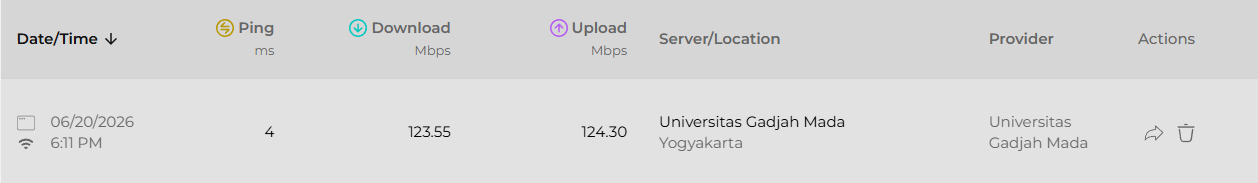
\includegraphics[width=0.9\textwidth]{contents/chapter-3/speedtest.png}
    \caption{Hasil pengujian kecepatan jaringan dengan \textit{Speedtest by Ookla} saat pengukuran.}
    \label{fig:speedtest}
\end{figure}

Pengujian pada kondisi nyata menemukan bahwa sebagian kamera publik dapat tidak aktif 
sewaktu-waktu. Pada implementasi awal, pembaca \textit{stream} dirancang untuk mencoba menyambung 
ulang tanpa batas, sehingga satu kamera yang tidak aktif membuat satu siklus pemrosesan 
tertahan hingga sistem dimulai ulang. Karena penjadwal latar belakang berjalan berurutan dalam satu 
utas, penundaan ini menghentikan pemantauan seluruh kamera lain selama itu. Masalah ini 
diatasi dengan menambahkan batas waktu pengambilan \textit{frame} sebesar 10 detik. Jika 
pengambilan melewati batas tersebut, proses dihentikan secara kooperatif dan giliran 
dilanjutkan ke kamera berikutnya, dengan status dicatat sebagai \textit{timeout}. Setelah 
perbaikan, satu kamera yang tidak aktif hanya menambah sekitar 10 detik pada satu putaran, 
sehingga dampak satu kamera mati tidak menghentikan keseluruhan proses inferensi kamera 
yang tidak sedang dipilih.

\subsection{Estimasi Kepadatan dan Ambang Notifikasi}

Notifikasi kepadatan didasarkan pada konsep \textit{Level of Service} (LOS) pejalan kaki, 
yang menyatakan tingkat kenyamanan suatu ruang pejalan kaki berdasarkan kepadatan orang 
per satuan luas \cite{fruin1971designing}. Standar serupa juga diatur dalam pedoman 
teknis penyediaan prasarana pejalan kaki di Indonesia \cite{pupr2014pedoman}. Penerapan 
LOS menuntut konversi dari jumlah orang yang terdeteksi pada citra menjadi kepadatan pada 
luas ruang nyata, yang dilakukan dengan membagi jumlah orang yang terdeteksi dengan luas 
area pejalan kaki yang tercakup kamera tersebut. Luas area diestimasi secara independen 
menggunakan fitur pengukuran pada \textit{Google Earth}, bukan dari koordinat piksel pada 
citra CCTV itu sendiri.

Pendekatan ini mensyaratkan sudut pandang kamera yang tetap, karena luas area yang 
diestimasi pada \textit{Google Earth} hanya berlaku selama batas area pejalan kaki yang 
tercakup kamera tidak berubah. Pada kenyataannya, sebagian kamera CCTV di kawasan ini 
memiliki sudut pandang yang tidak tetap, sebagian di antaranya dapat digerakkan, sebagaimana 
ditunjukkan pada Gambar \ref{fig:kamera_ptz} yang memperlihatkan kamera yang sama pada sudut 
yang berbeda. Oleh karena itu, kalibrasi LOS berbasis estimasi luas ini hanya diterapkan 
pada dua kamera yang sudut pandangnya relatif tetap sebagai contoh penerapan, sedangkan 
ambang untuk kamera lain ditentukan secara manual. Pembatasan ini sejalan dengan batasan 
penelitian yang diuraikan pada Bab I.

\begin{figure}[htbp]
    \centering
    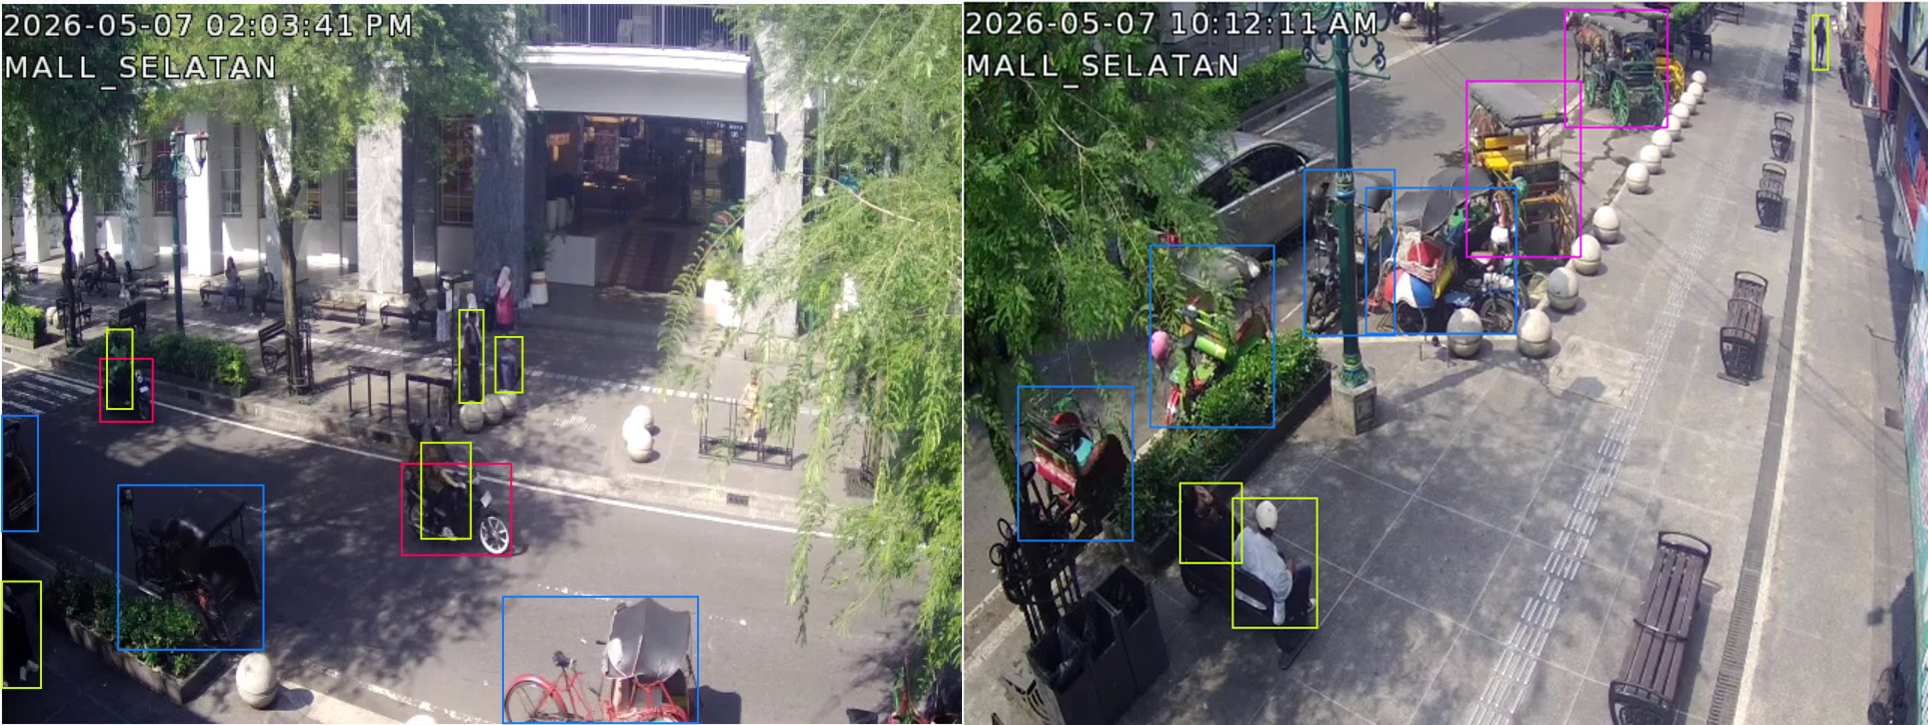
\includegraphics[width=0.9\textwidth]{contents/chapter-3/buktidinamis.png}
    \caption{Kamera CCTV yang sama pada dua sudut pandang berbeda}
    \label{fig:kamera_ptz}
\end{figure}

Pemilihan dua kamera tersebut sebagai titik kalibrasi LOS tidak semata karena sudut 
pandangnya relatif tetap. Kedua kamera juga mengarah ke segmen trotoar yang cukup luas dan 
terbuka, sehingga dimensi ruang nyatanya dapat diestimasi dengan andal melalui pengukuran 
pada \textit{Google Earth}. Selain itu, kedua titik 
tersebut termasuk lokasi yang kerap menjadi pusat keramaian di koridor Malioboro, sehingga 
estimasi kepadatan di sana paling relevan untuk tujuan pemantauan dan pengendalian 
kerumunan.

Kamera pertama mengarah ke area pejalan kaki di seberang Gedung Agung, sebagaimana 
ditunjukkan pada Gambar \ref{fig:kamera_ga}. Estimasi dengan fitur \textit{measurement} pada 
\textit{Google Earth} menghasilkan luas area pejalan kaki yang tercakup kamera tersebut 
sekitar 169~m\textsuperscript{2}, sebagaimana terlihat pada Gambar \ref{fig:ukur_ga}. 
Luas inilah yang menjadi penyebut dalam mengubah jumlah orang yang terdeteksi menjadi 
kepadatan per meter persegi pada titik tersebut.

Kamera kedua mengarah ke area pejalan kaki Titik Nol yang menghadap ke utara, sebagaimana 
ditunjukkan pada Gambar \ref{fig:kamera_tn}. Pengukuran serupa pada \textit{Google Earth} 
menghasilkan luas area pejalan kaki yang tercakup sekitar 149~m\textsuperscript{2}, 
sebagaimana terlihat pada Gambar \ref{fig:ukur_tn}. Dengan luas kedua zona yang telah 
diketahui, jumlah orang pada masing-masing kamera dapat diubah menjadi nilai kepadatan dan 
dipetakan ke tingkat pelayanan pada Tabel \ref{tab:los}, dan ambang notifikasi yang 
diturunkan dari kedua luas tersebut disajikan pada Bab IV bersama hasil pengujian sistem.

Estimasi luas melalui \textit{Google Earth} ini perlu diakui memiliki keterbatasan. 
Pengukuran tersebut tidak divalidasi dengan pengukuran fisik langsung di lapangan, seperti 
menggunakan meteran atau alat ukur jarak lainnya pada kedua titik kamera, sehingga nilai 
169~m\textsuperscript{2} dan 149~m\textsuperscript{2} adalah estimasi visual, bukan hasil 
pengukuran terverifikasi. Sumber kesalahan yang mungkin muncul antara lain distorsi 
perspektif citra satelit yang digunakan \textit{Google Earth}, yang berbeda dengan 
distorsi perspektif sudut pandang miring kamera CCTV, serta ketidaktepatan dalam menentukan 
batas tepi area pejalan kaki secara visual pada kedua jenis citra tersebut. Meskipun 
demikian, pendekatan ini dipandang sebagai solusi yang masuk akal pada lingkup dan sumber 
daya penelitian ini, mengingat tidak tersedia akses untuk survei lapangan langsung pada 
kedua titik kamera, dan estimasi visual tetap memberikan dasar kuantitatif yang lebih baik 
dibanding penentuan ambang notifikasi secara sepenuhnya manual tanpa rujukan luas area sama 
sekali. Validasi lapangan terhadap estimasi ini diajukan sebagai arah pengembangan lanjutan 
pada Bab V.

\begin{figure}[htbp]
    \centering
    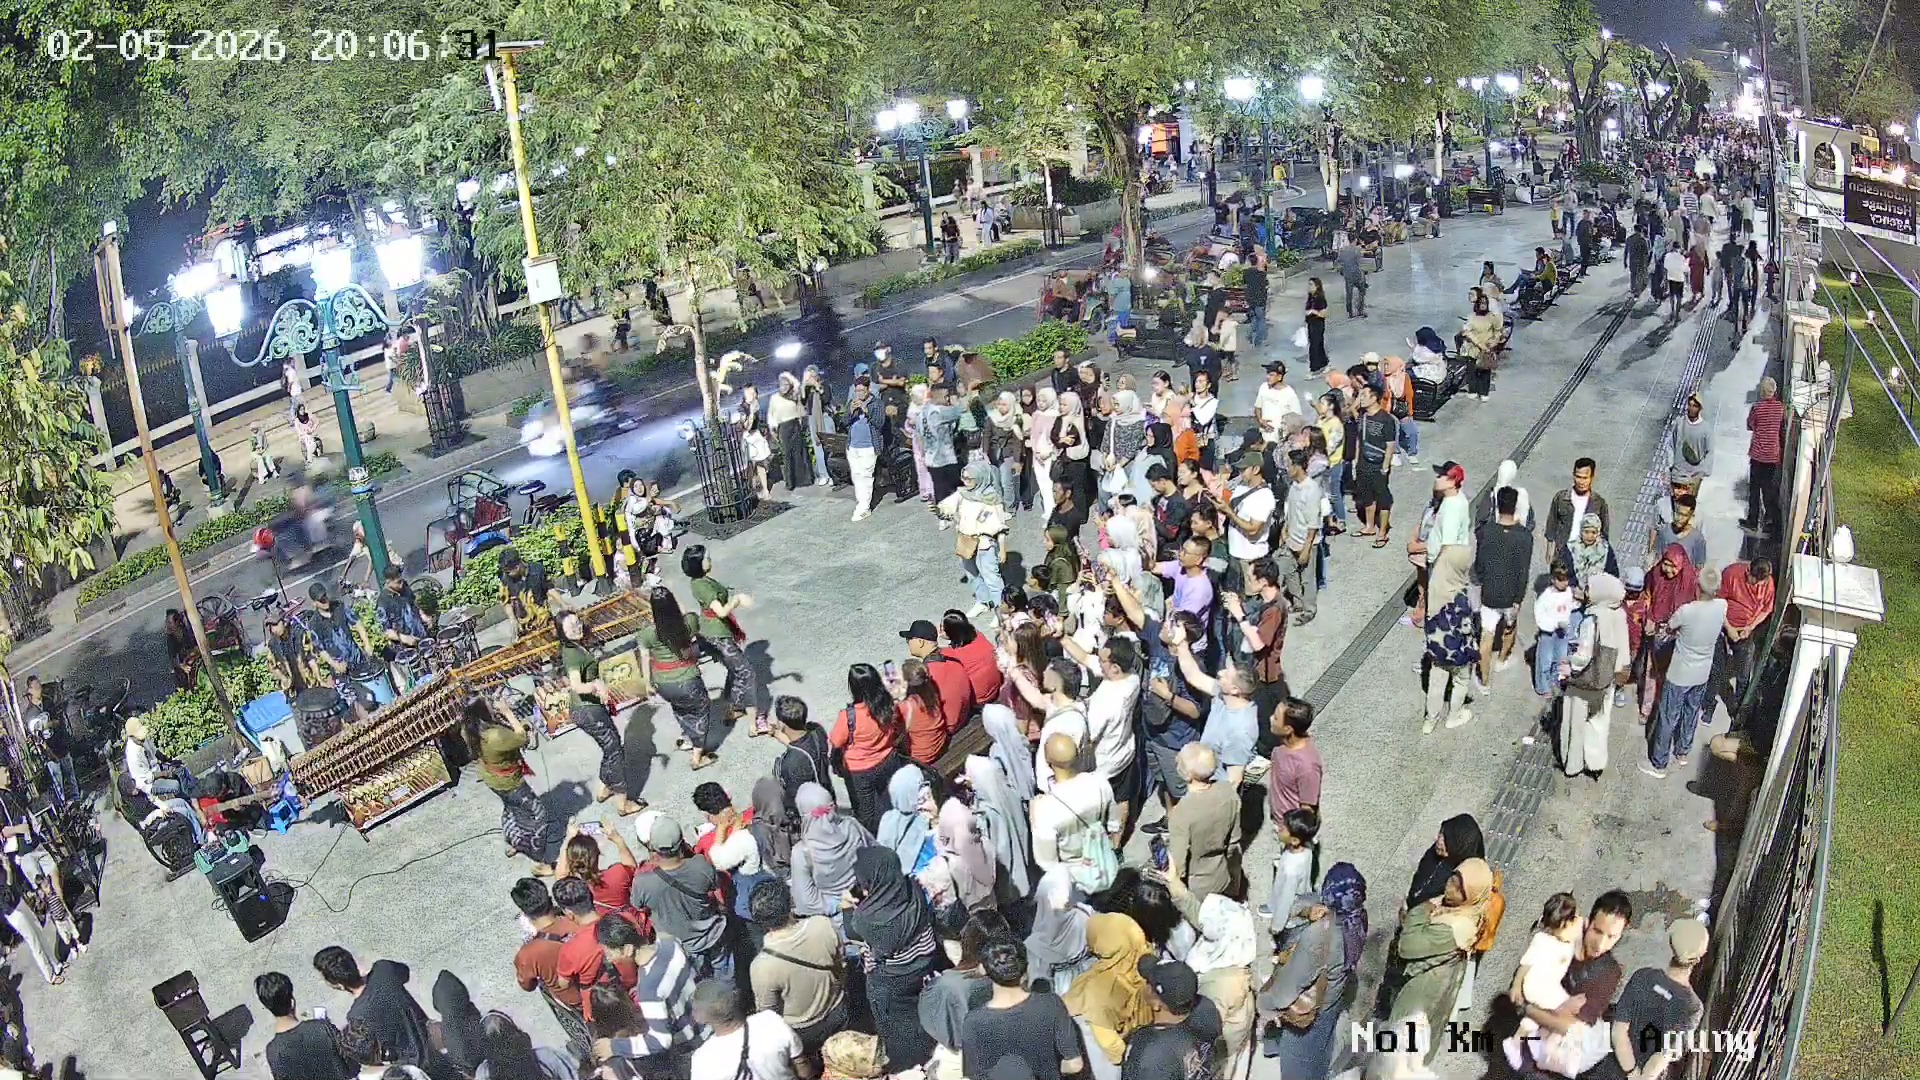
\includegraphics[width=0.9\textwidth]{contents/chapter-3/cam19_Nol_KM_Gedung_Agung.jpg}
    \caption{Citra CCTV area pejalan kaki di seberang Gedung Agung.}
    \label{fig:kamera_ga}
\end{figure}

\begin{figure}[htbp]
    \centering
    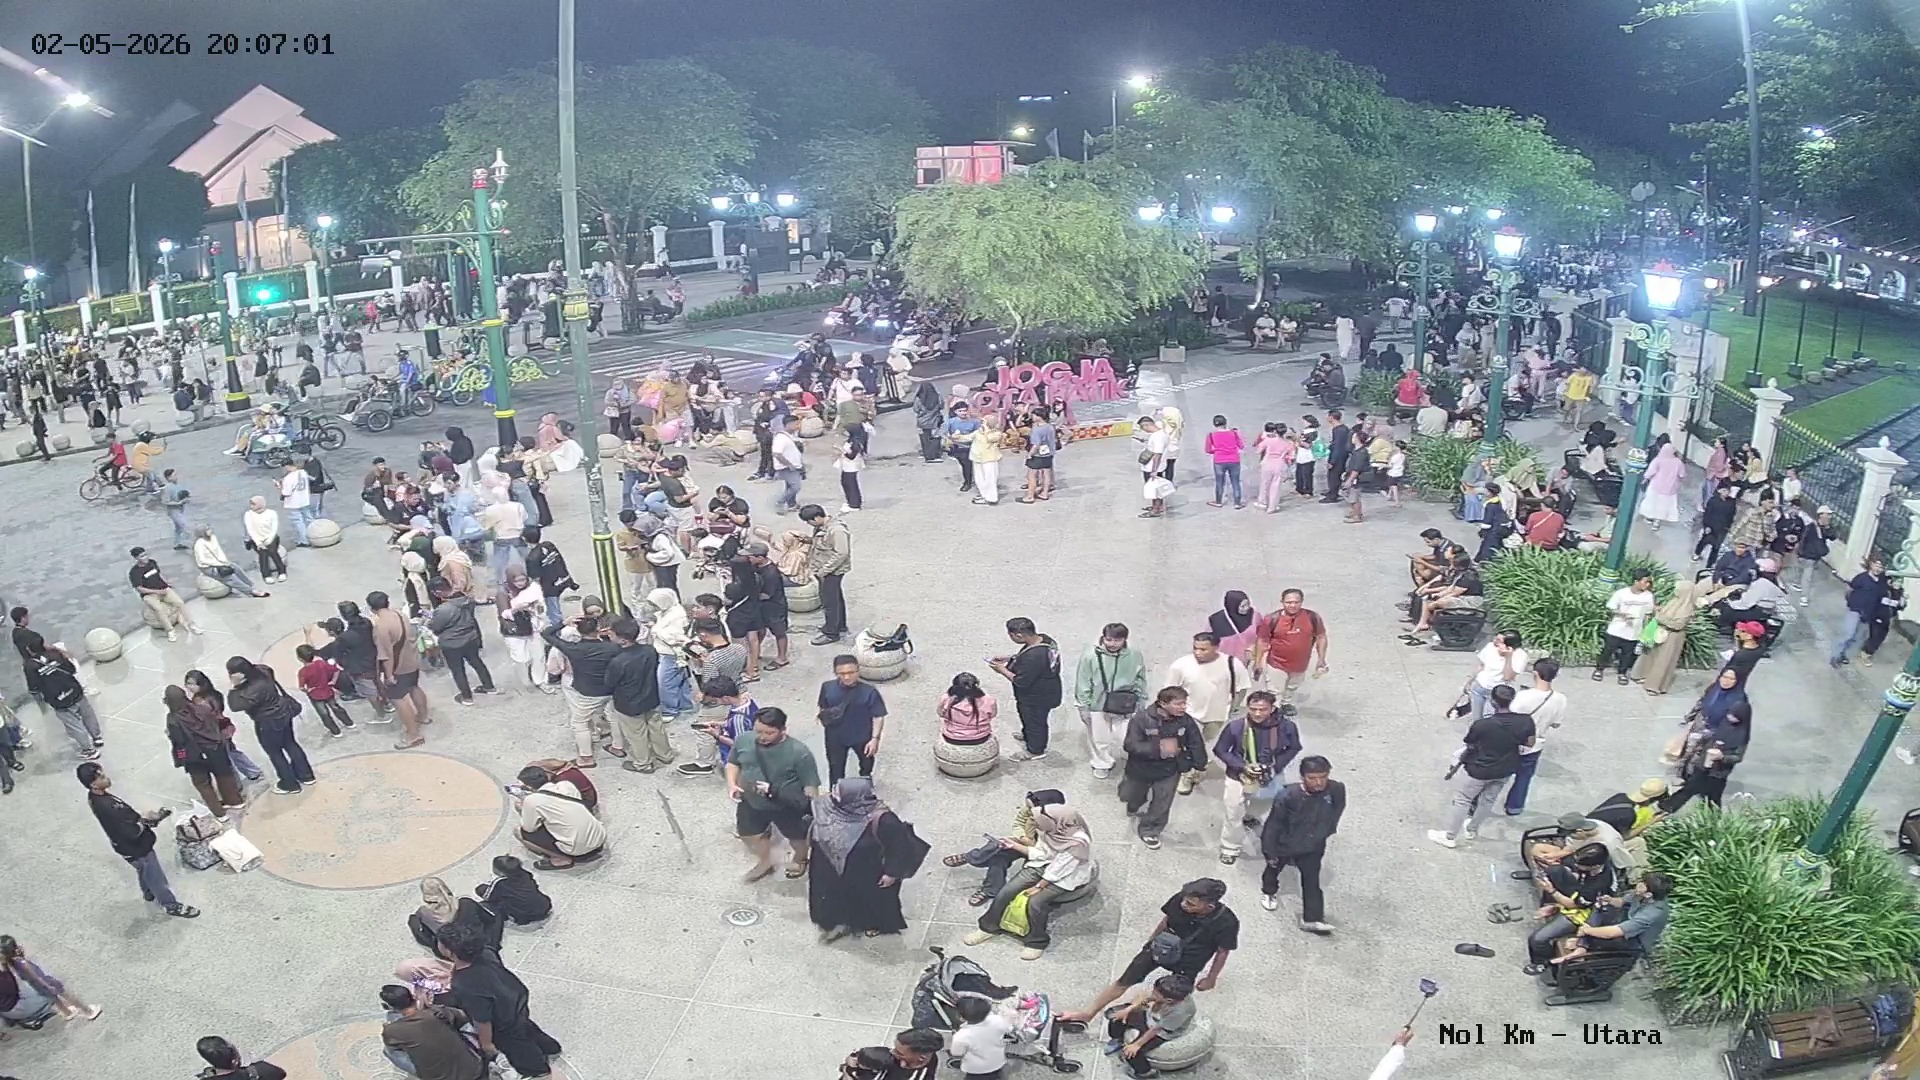
\includegraphics[width=0.9\textwidth]{contents/chapter-3/cam20_Nol_KM_Utara.jpg}
    \caption{Citra CCTV area pejalan kaki Titik Nol yang menghadap ke utara.}
    \label{fig:kamera_tn}
\end{figure}

\begin{figure}[htbp]
    \centering
    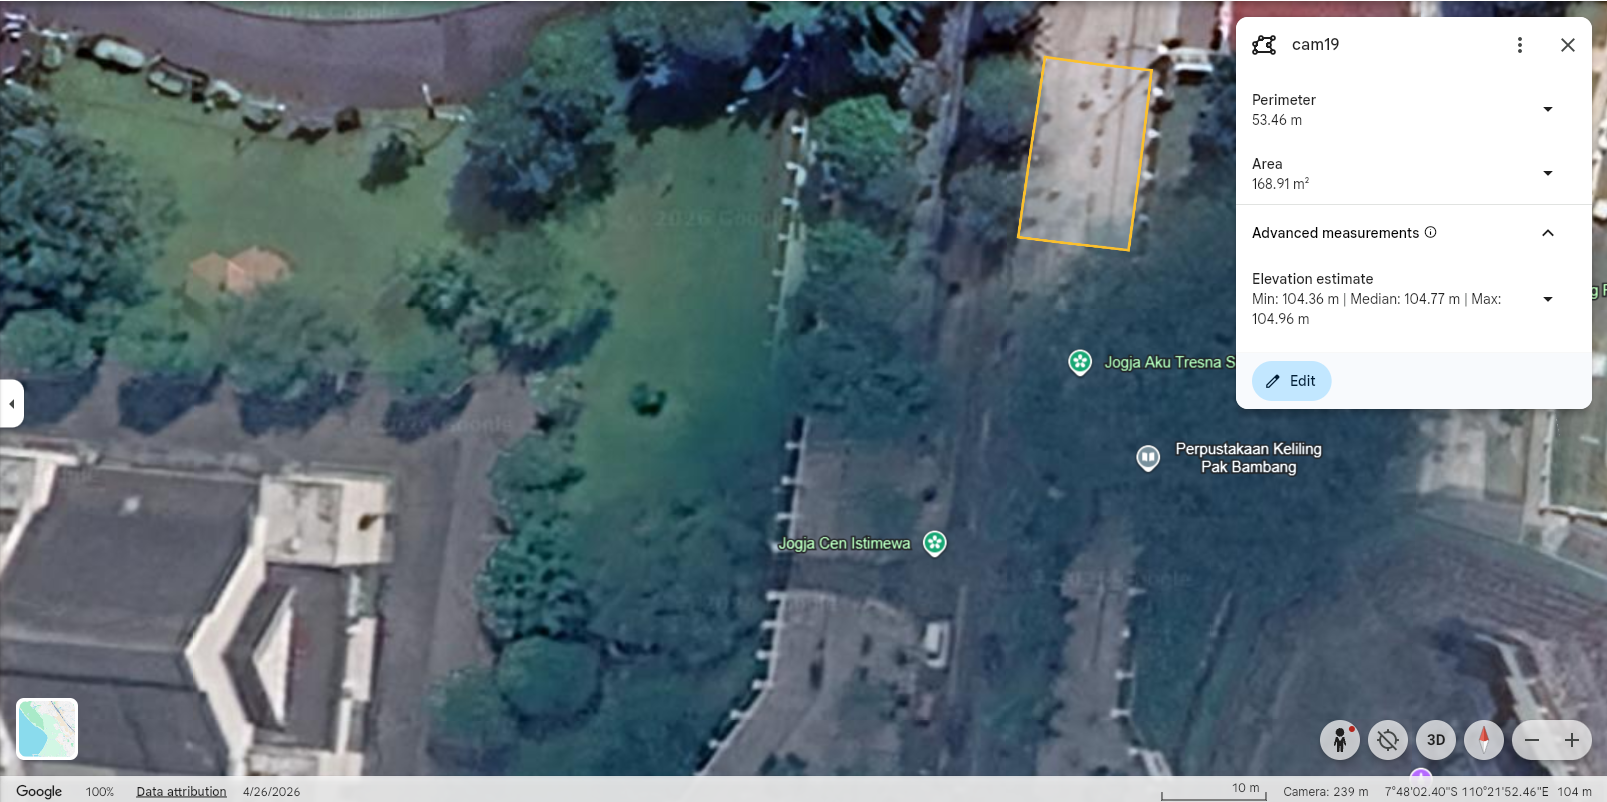
\includegraphics[width=0.9\textwidth]{contents/chapter-3/LOS_cam19.png}
    \caption{Pengukuran luas area pejalan kaki yang tercakup CCTV seberang Gedung Agung pada \textit{Google Earth}.}
    \label{fig:ukur_ga}
\end{figure}

\begin{figure}[htbp]
    \centering
    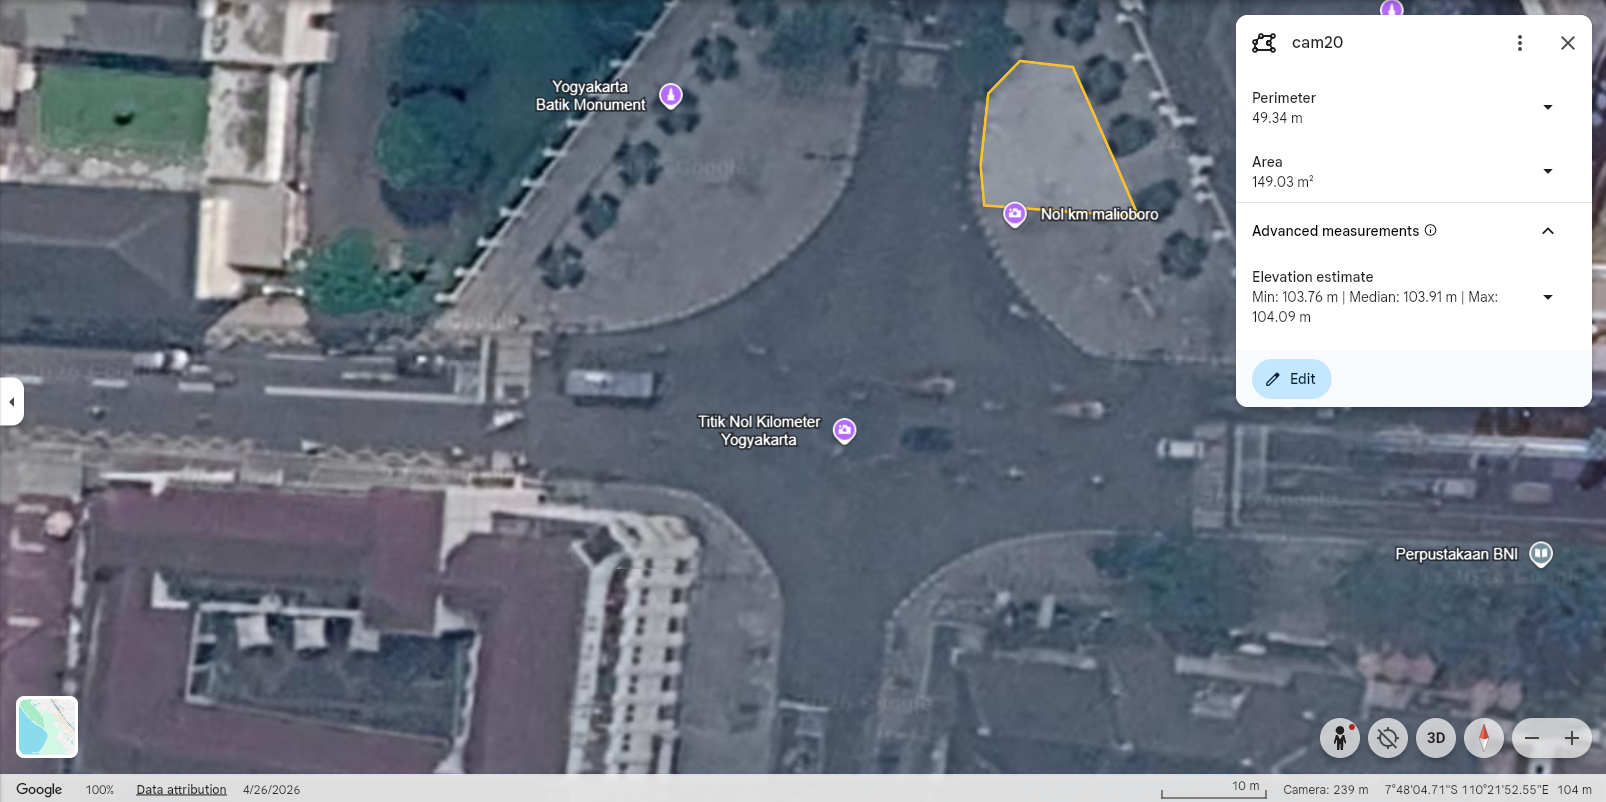
\includegraphics[width=0.9\textwidth]{contents/chapter-3/LOS_cam20.png}
    \caption{Pengukuran luas area pejalan kaki yang tercakup CCTV Titik Nol pada \textit{Google Earth}.}
    \label{fig:ukur_tn}
\end{figure}

Alasan yang sama, yaitu sudut pandang yang dapat bergeser seperti diperlihatkan pada 
Gambar \ref{fig:kamera_ptz}, juga mendasari keputusan untuk tidak menggunakan area pemantauan 
terbatas (\textit{Region of Interest}). Poligon area yang digambar satu kali tidak lagi sahih setelah 
kamera bergeser, sehingga penghitungan objek dilakukan pada seluruh \textit{frame}, bukan 
pada area terbatas tertentu. Penghitungan pada seluruh \textit{frame} memang mengorbankan 
kemampuan membatasi zona, tetapi menjamin hasil tetap konsisten meskipun sudut pandang kamera 
berubah.

Ambang notifikasi ditetapkan per kelas untuk tiap kamera, bukan sebagai satu ambang 
tunggal yang berlaku sama untuk seluruh kamera. Hal ini diperlukan karena tiap titik 
kamera mewakili ruang dengan kapasitas yang berbeda, sehingga jumlah objek yang menandakan 
kepadatan berlebih pun berbeda antarlokasi. Untuk dua kamera yang terkalibrasi LOS, 
ambang jumlah orang diturunkan dari kapasitas ruang hasil estimasi luas pada \textit{Google 
Earth}. Untuk kamera lainnya, ambang ditentukan secara manual. Nilai ambang ini disimpan 
dalam berkas konfigurasi tiap kamera.

Agar notifikasi tidak terkirim berulang kali selama kondisi padat masih berlangsung, 
sistem menerapkan tenggang waktu antarnotifikasi untuk kombinasi kamera dan jenis 
notifikasi yang sama. Tenggang waktu ditetapkan selama 7 menit, yang dinilai cukup untuk 
mencegah notifikasi yang berlebihan tanpa membuat sistem lambat menanggapi kondisi yang 
dapat berubah cepat. Jika kepadatan melonjak jauh melampaui ambang, tenggang waktu ini 
diabaikan agar kondisi yang lebih berbahaya tetap diberitahukan. Penetapan nilai tenggang 
waktu ini adalah pertimbangan rekayasa, bukan mengikuti standar tertentu.

Selain dikirim sebagai notifikasi, tiap peringatan yang melampaui ambang juga disimpan 
beserta citra CCTV pada saat peringatan terpicu dan kotak deteksi yang menyertainya, 
sehingga operator dapat meninjaunya kembali melalui halaman riwayat peringatan. Citra 
disimpan dalam bentuk asli tanpa anotasi, sedangkan kotak deteksi digambar ulang dari 
data koordinat yang tersimpan saat citra ditampilkan, agar penyimpanan tetap hemat tanpa 
menggandakan berkas gambar. Riwayat ini membuat peringatan tidak sekadar lewat sesaat, 
melainkan terdokumentasi sebagai bukti kondisi kepadatan yang dapat diperiksa ulang.

\subsection{Visualisasi Kepadatan pada Dashboard}

Antarmuka menyajikan grafik kepadatan yang merangkum riwayat deteksi tiap kamera. Metrik 
yang ditampilkan secara khusus adalah jumlah orang, bukan gabungan seluruh kelas objek, 
karena penggabungan orang dan kendaraan menjadi satu angka akan kehilangan makna mengingat 
skala kepadatan keduanya berbeda. Selain itu, dasar notifikasi dan tingkat pelayanan (LOS) 
pada penelitian ini khusus berlaku untuk pejalan kaki, sehingga grafik kepadatan pada 
\textit{dashboard} difokuskan pada kelas orang agar selaras dengan dasar teori tersebut. 
Jumlah objek kelas kendaraan tetap tersimpan pada riwayat deteksi untuk kemungkinan 
pemanfaatan lebih lanjut, tetapi tidak ditampilkan pada grafik kepadatan saat ini.

Riwayat deteksi tidak disimpan per \textit{frame}, melainkan diringkas setiap lima menit 
untuk tiap kamera. Pada tiap jendela lima menit, sistem mencatat dua besaran untuk kelas 
orang, yaitu rata-rata jumlah orang dari seluruh \textit{frame} yang terkumpul sebagai 
gambaran kondisi tipikal, dan nilai puncak berupa jumlah orang tertinggi pada satu 
\textit{frame} di dalam jendela tersebut sebagai penanda lonjakan sesaat. Pemisahan ini 
diperlukan karena untuk tujuan keselamatan momen puncak kepadatan lebih penting daripada 
rata-rata yang dapat menutupi lonjakan singkat. Penyajian tren semacam ini menjadi 
representasi standar pada pemantauan kerumunan, sebagaimana ditunjukkan pada platform 
pemantauan transit yang menampilkan variasi jumlah orang sepanjang hari 
\cite{apeksha2025transit}, dan membantu operator memahami kondisi kepadatan tanpa harus 
mengamati seluruh kamera secara manual yang melelahkan serta rawan kesalahan 
\cite{wong2024fusion}.

Pengguna dapat memilih dua rentang waktu, dan keduanya menampilkan baik rata-rata maupun 
puncak jumlah orang. Rentang harian menampilkan tren per jam pada satu tanggal terpilih, 
dengan nilai tiap jam dihitung dari ringkasan lima-menitan yang jatuh pada jam tersebut. 
Rentang mingguan menampilkan tren per hari selama tujuh hari kalender terakhir, dengan nilai 
tiap hari dihitung dari seluruh ringkasan lima-menitan pada hari tersebut. Seluruh 
pengelompokan jam dan hari menggunakan zona waktu setempat (WIB), dan grafik disajikan 
terpisah untuk tiap kamera karena tiap lokasi memiliki karakter kepadatan yang berbeda.

Granularitas dasar visualisasi ini adalah ringkasan lima menit, sehingga rata-rata maupun 
puncak per jam dan per hari dihitung dari ringkasan tersebut, bukan langsung dari tiap 
\textit{frame}. Selain itu, rata-rata lima-menitan dihitung tanpa pembobotan waktu terhadap 
perbedaan laju pengambilan \textit{frame} antara kamera aktif dan kamera latar belakang, 
sehingga nilainya lebih mencerminkan rata-rata atas sampel yang terkumpul daripada rata-rata 
atas durasi. Keterbatasan ini tidak memengaruhi fungsi pemantauan, tetapi perlu diperhatikan 
bila data digunakan untuk analisis kuantitatif lebih lanjut.